\section{Quick look at simulation result: net2g} \label{sec:quicklook}
%####################################################################################

In this section, we explain how to use netcdf2grads. The program netcdf2grads (for short, net2g) merges the \netcdf files (\verb|history.**.nc|)\footnote{If ``gpview'' is installed, it can also be used for drawing. This tool is more suitable for quick check  because it is available without the conversion of history data.},  which are divided process by process, into a binary file in \grads format. The simulation results are also validated using the converted \grads binary data.

\subsubsection{Conversion to \grads binary}
%-----------------------------------------------------------------------------------
Use \verb|net2g| to convert \grads binary from the history file of \netcdf having divided every process.  Only a minimum of the procedures is explained here.  Refer to Section \ref{sec:net2g} for their detailed use.

First, move to the directory \verb|net2g|:
\begin{verbatim}
 $ cd ${Tutorial_DIR}/real/experiment/net2g
 $ ls
    net2g -> ../../../../../util/netcdf2grads_h/net2g
    net2g.2D.d01.conf
    net2g.3D.d01.conf
\end{verbatim}
There are some configuration files and a binary file in this directory.  The binary file is linked to the executable file compiled in Section \ref{sec:source_net2g}. As an example,  a procedure to convert the 2D variables MSLP and PREC to \grads format is explained here. We also explain how to extract the 3D variables U and V at 850 hPa, 500 hPa, and 200 hPa, and convert them into \grads format.  The configuration files for 2D and 3D variables  are prepared as files \verb|net2g.3D.d01.conf| and \verb|net2g.2D.d01.conf|, respectively. 
 
When \verb|net2g| is executed, the number of processes needs to be a divisor of the number of the processes used for the simulation. 
The number of processes is four here. Since \verb|net2g| cannot simultaneously convert 2D and 3D variables , they must be converted separately as follows:
\begin{verbatim}
 $ mpirun -n 4 ./net2g net2g.2D.d01.conf
 $ mpirun -n 4 ./net2g net2g.3D.d01.conf
\end{verbatim}
The conversion succeeds only if the following messages are found  in the standard output without an error message:
\msgbox{
\verb|+++ MPI COMM: Corrective Finalize| \\
}
The following files are also found. \verb|**.ctl| represents the ``ctl'' file for the XY grid system of \scalerm, \verb|**lccr.ctl| a ctl file for the drawing results on the latitude-longitude coordinates:
\begin{verbatim}
  MSLP_d01z-2d.ctl
  MSLP_d01z-2d.grd
  MSLP_d01z-2d_lccr.ctl
  PREC_d01z-2d.ctl
  PREC_d01z-2d.grd
  PREC_d01z-2d_lccr.ctl
  PRES_d01z-3d.ctl
  PRES_d01z-3d.grd
  PRES_d01z-3d_lccr.ctl
  U_d01z-3d.ctl
  U_d01z-3d.grd
  U_d01z-3d_lccr.ctl
  V_d01z-3d.ctl
  V_d01z-3d.grd
  V_d01z-3d_lccr.ctl
\end{verbatim}


\subsubsection{Validation of simulation result}
%-----------------------------------------------------------------------------------
Confirm the calculation results using a \grads script \verb|checkfig_real.gs|: 
\begin{verbatim}
 $ cp ../../data/checkfig_real.gs ./
 $ grads -blc checkfig_real.gs
\end{verbatim}
The following files are generated when the conversion is successfully finished. Note that the script changes accordingly when a warning appears. This is because the syntax is different according to the version of \grads.
\begin{verbatim}
  real_mslp.png
  real_prec.png
  real_wind.png
\end{verbatim}
If the calculation are successful, the same figures as Figs. \ref{fig:real_mslp}, \ref{fig:real_prec}, and \ref{fig:real_wind}  are obtained.

\begin{figure}[tbh]
\begin{center}
  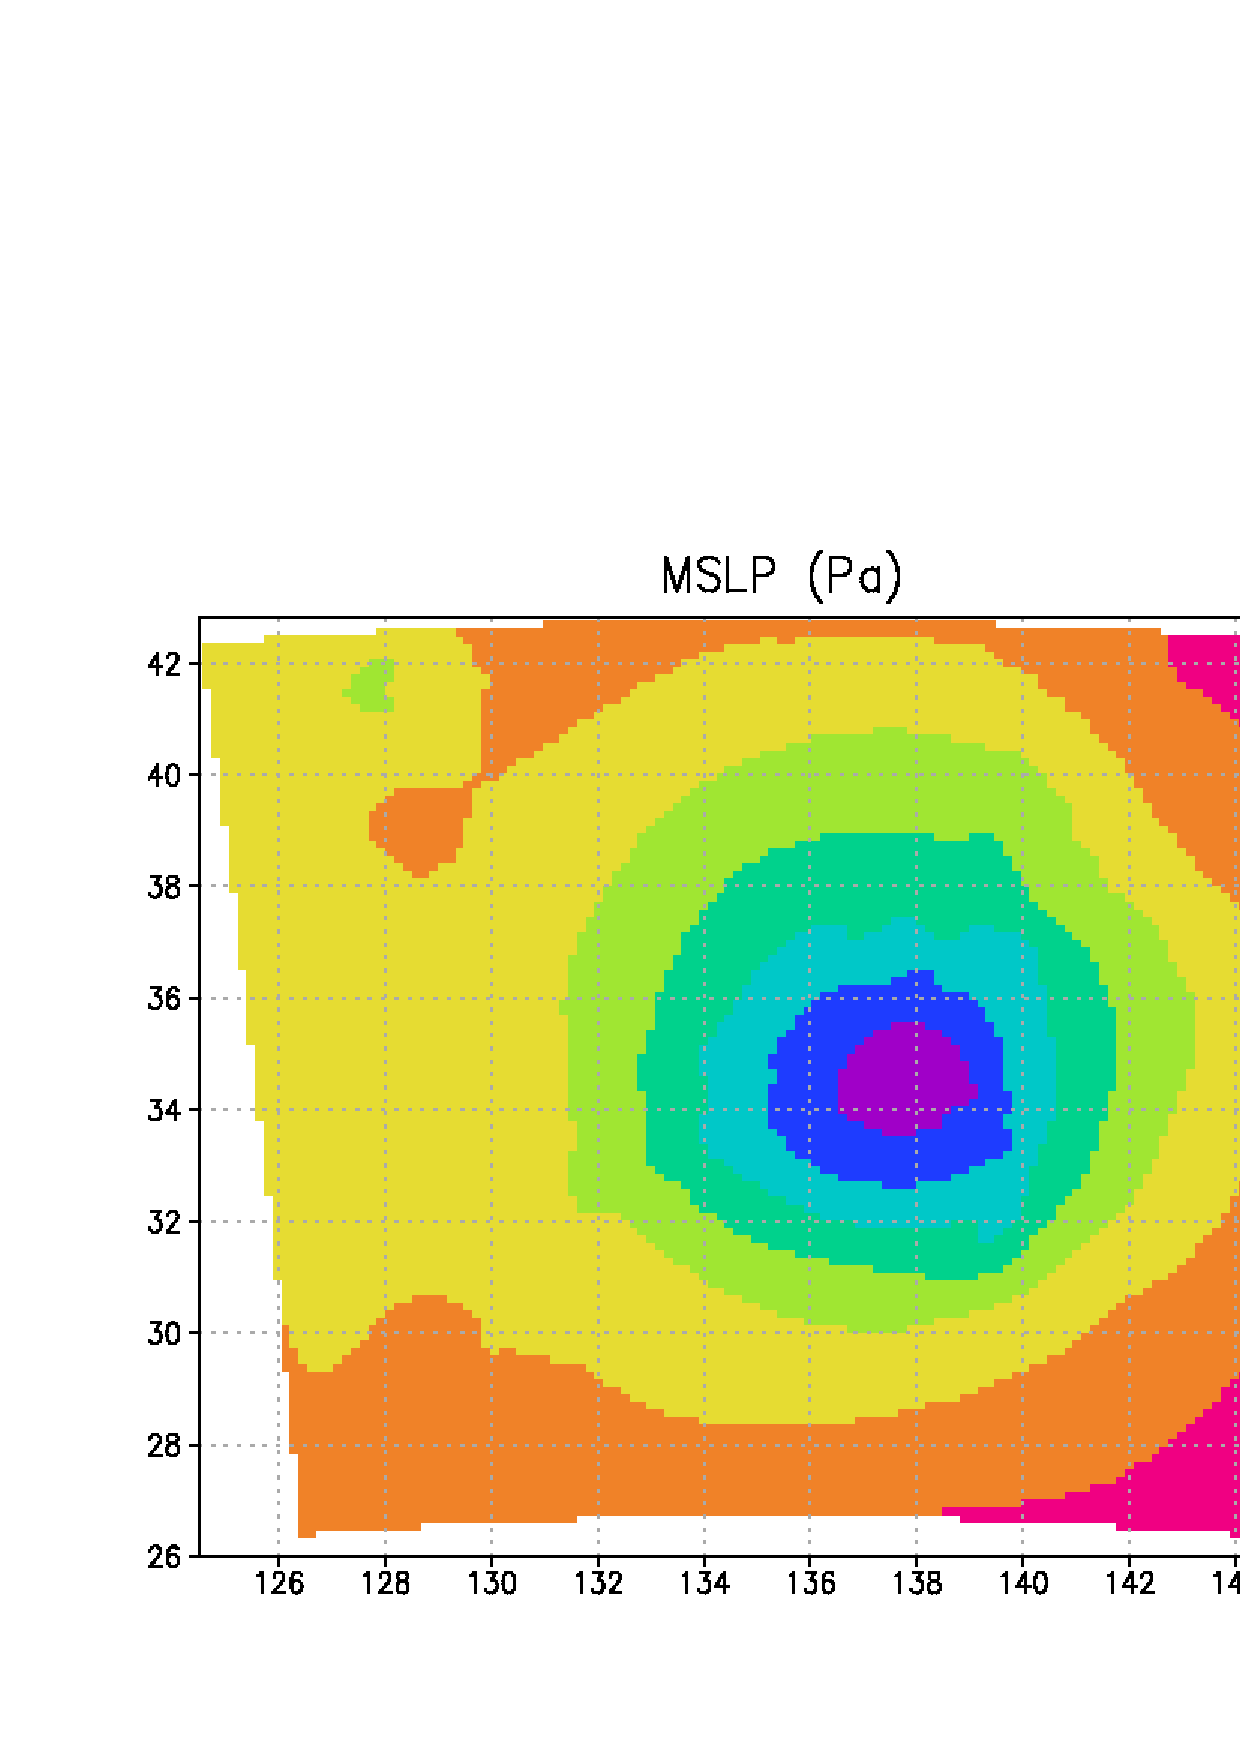
\includegraphics[width=0.55\hsize]{./figure/real_mslp.pdf}\\
  \caption{Sea-level pressure after 6 hours}
  \label{fig:real_mslp}
\end{center}
\begin{center}
  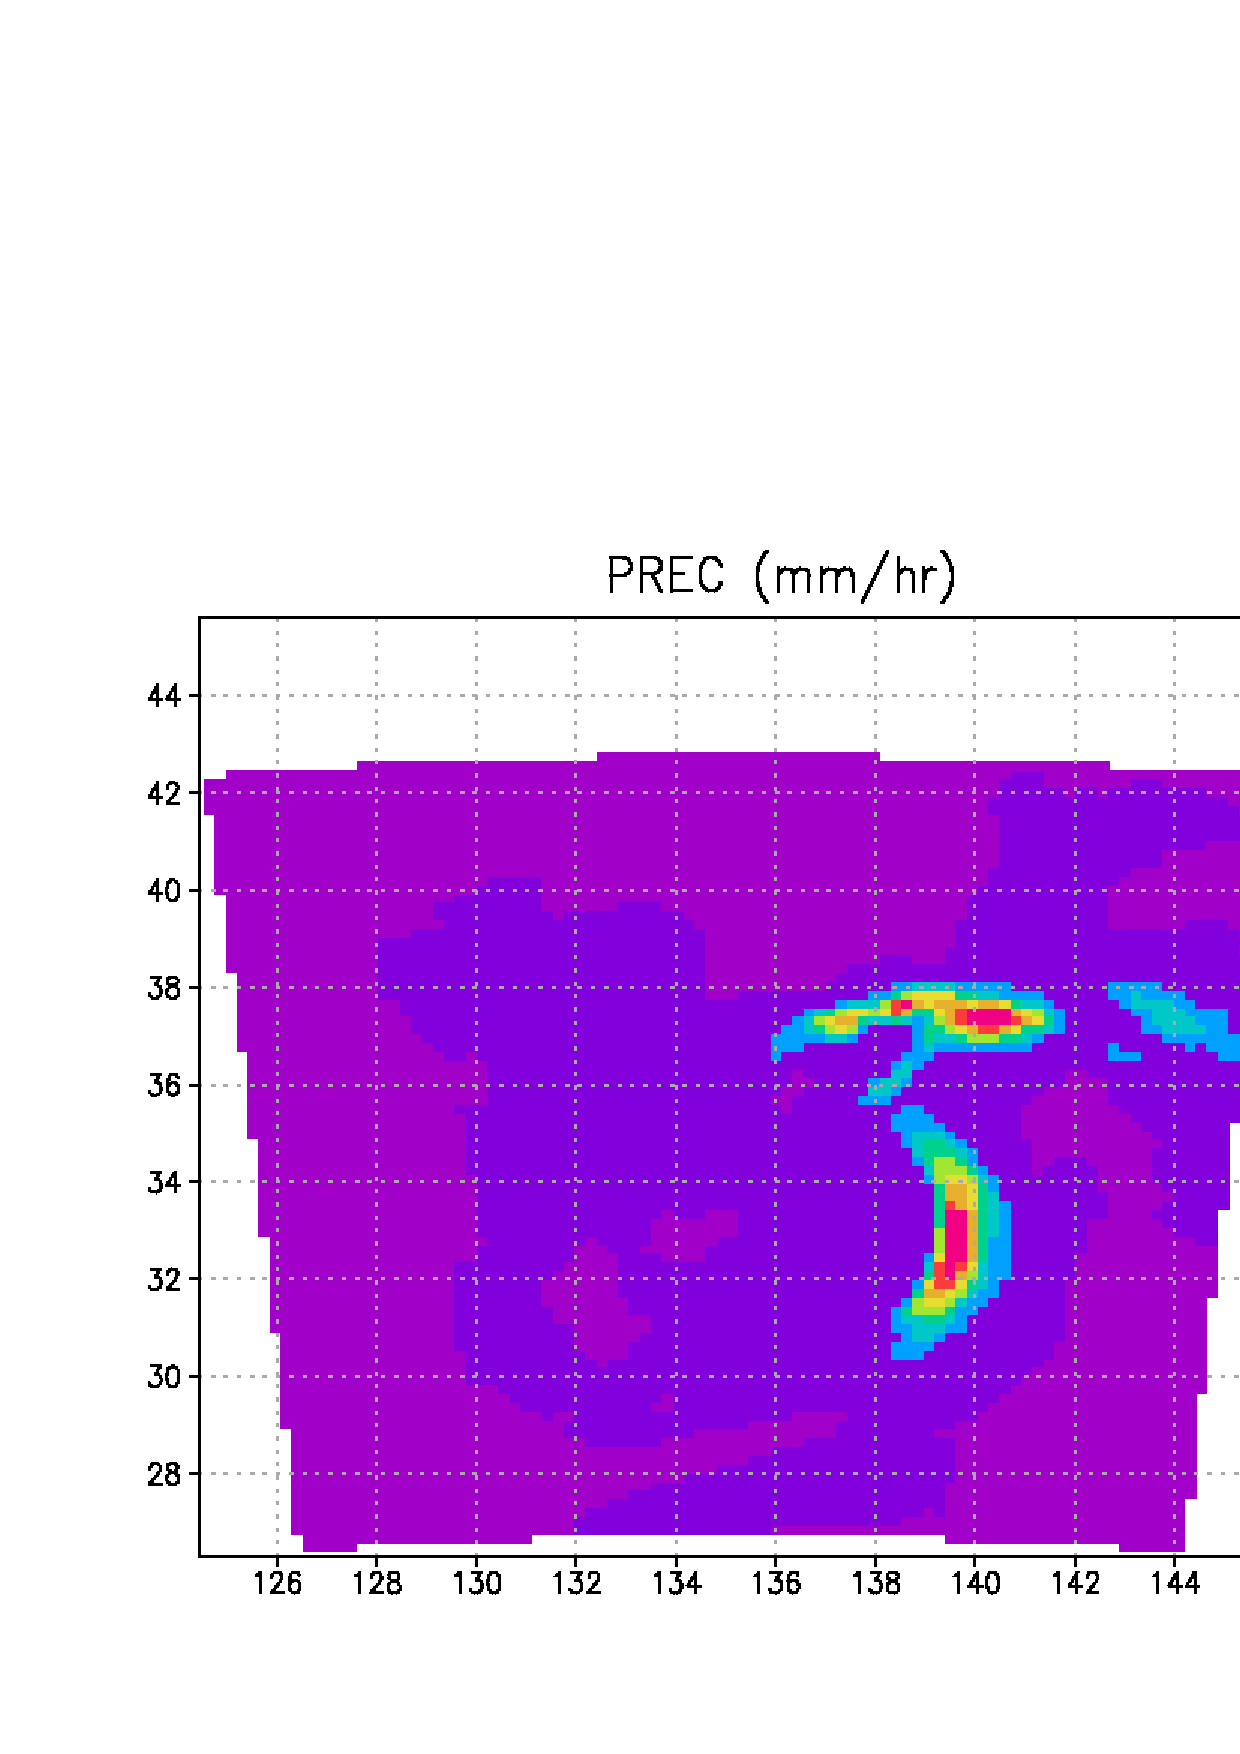
\includegraphics[width=0.55\hsize]{./figure/real_prec.pdf}\\
  \caption{Precipitation flux after 6 hours}
  \label{fig:real_prec}
\end{center}
\begin{center}
  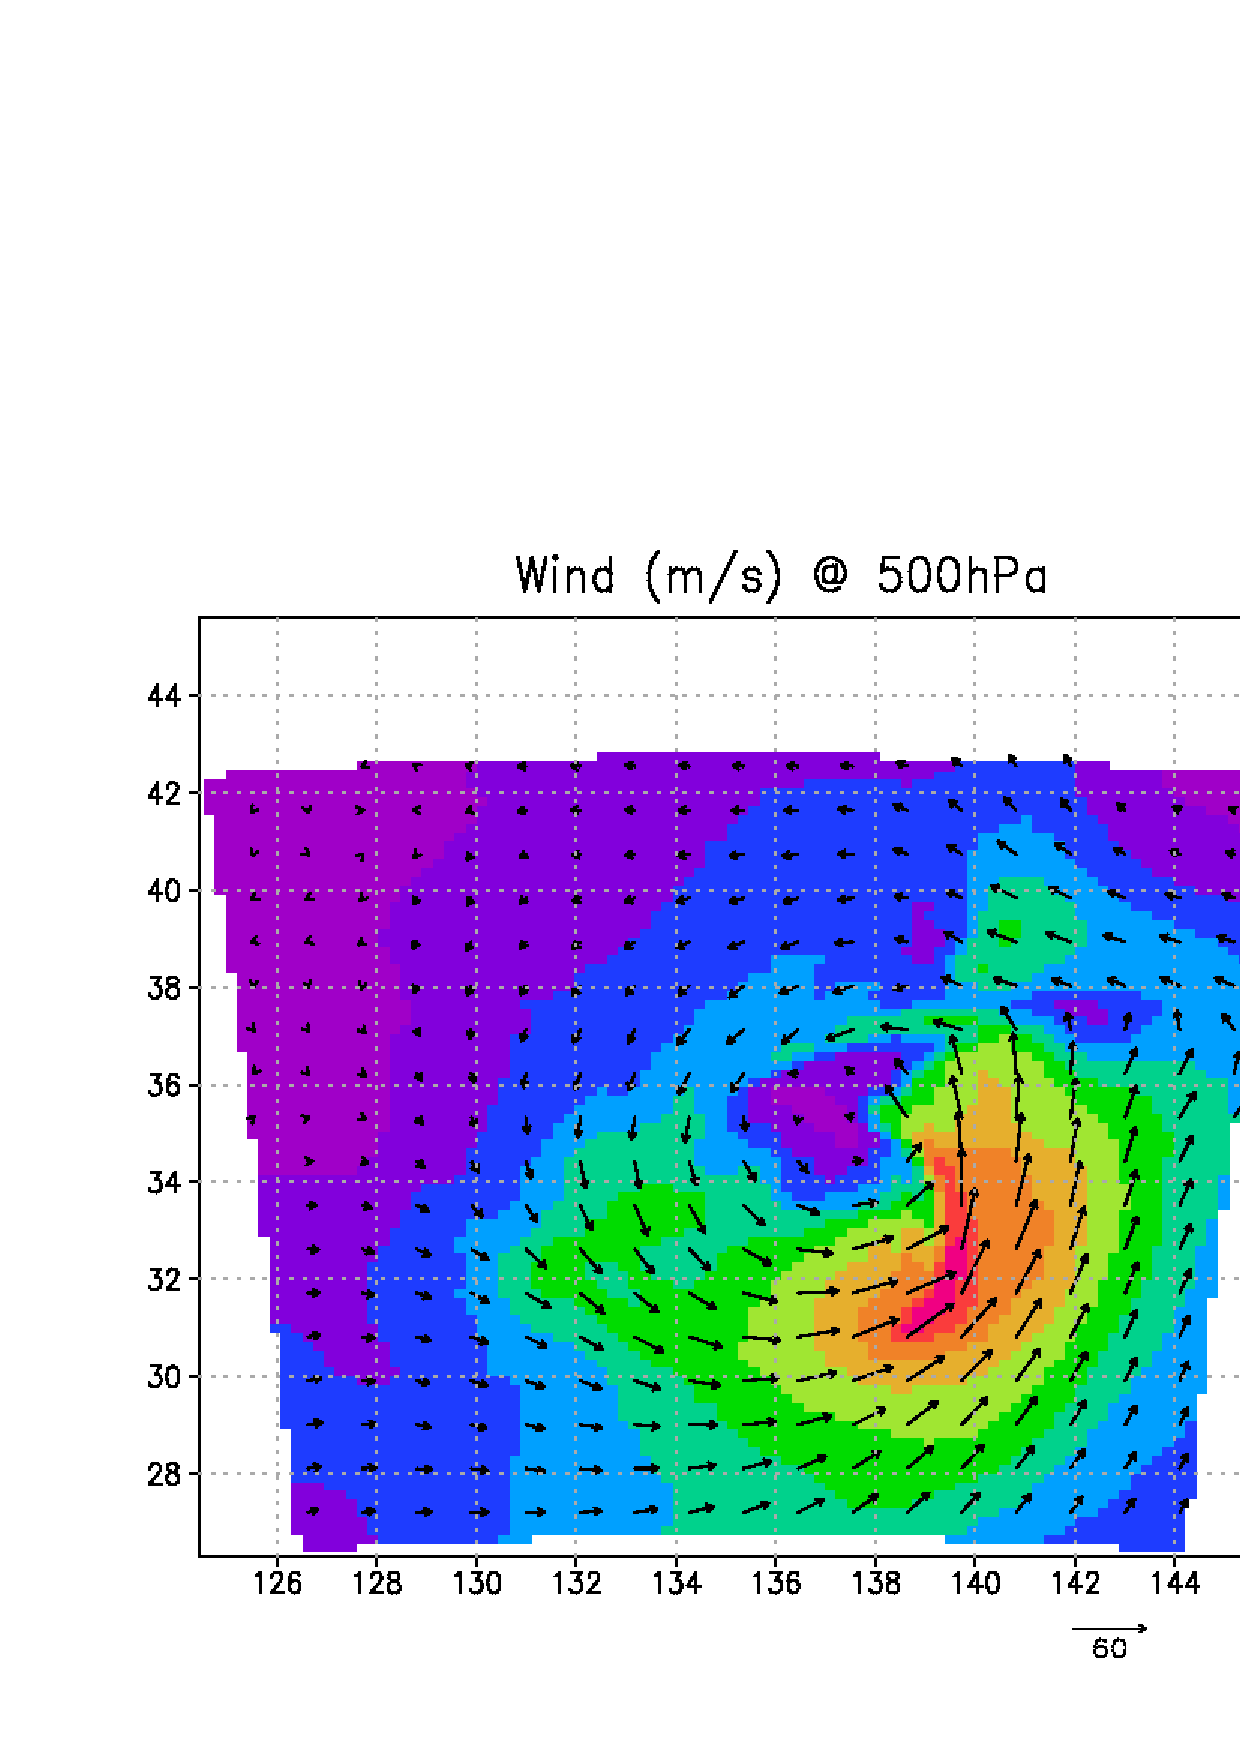
\includegraphics[width=0.55\hsize]{./figure/real_wind.pdf}\\
  \caption{Wind velocity after 6 hours}
  \label{fig:real_wind}
\end{center}
\end{figure}

